\section{Low-Level Planner}

The low-level planner's main task is to generate the goal poses the robot should drive to to execute the current high-level task. With the exception of the move through doorway task all those tasks are executed within a single room. Therefore the low-level planner can ignore other rooms to make the planning easier. In addition the low-level planner uses the results of the object detection to decide if an object of the searched type is found. This section gives an overview on how those tasks are planned and executed.

\subsection{Move Through Doorway Task}

The goal of this task is to drive through a specified doorway into the next room. It is the only high-level task, where the robot can drive into another room. The execution of this task is illustrated in figure \ref{fig:move_trough_doorway}. In a first step the robot is sent to a position in front of the doorway facing towards the doorway. In this process the door pose becomes more accurate and possible obstacles behind the doorway are detected. In a second step the robot is sent to a goal behind the doorway. When the robot passes the doorway the map is switched. During the execution the low-level planner keeps track of the doorway pose and changes the goal pose accordingly. This is especially important when the map switch occurs as the doorway pose can be completely different in the new rooms map coordinate frame. 

\begin{figure}[h]
\centering
  \subfloat[align in front of doorway]{{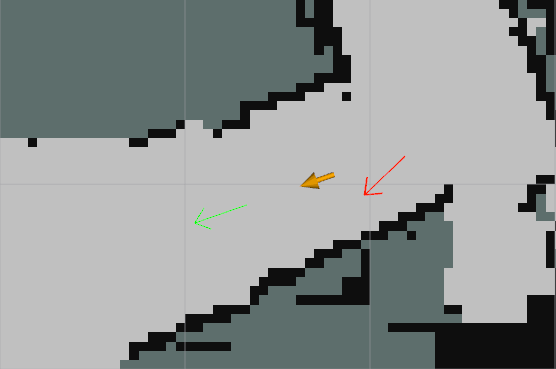
\includegraphics[width=0.3\textwidth]{figures/move_trough_doorway1.png} }}%
  \quad
  \subfloat[set goal behind doorway]{{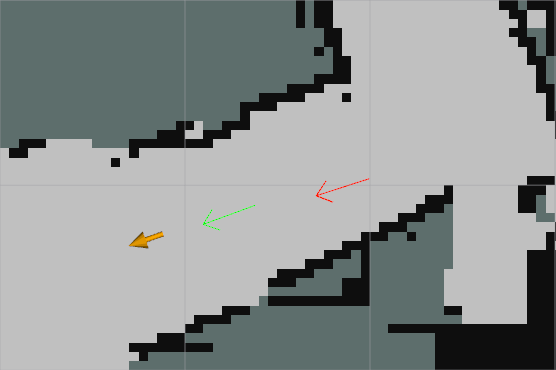
\includegraphics[width=0.3\textwidth]{figures/move_trough_doorway2.png} }}%
  \quad
  \subfloat[finish after map switch]{{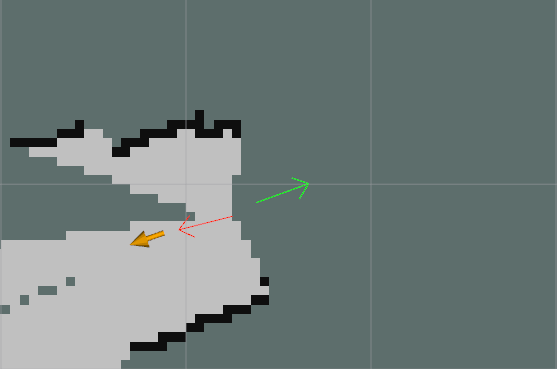
\includegraphics[width=0.3\textwidth]{figures/move_trough_doorway3.png} }}%
  \caption[Move through doorway task]{The three steps of the move through doorway task: The robot pose is in red, the current goal pose is in orange and the door pose is in green}
  \label{fig:move_trough_doorway} 
\end{figure}

\subsection{Peek Task}

The purpose of this task is to quickly get a first impression of a room never visited before. This is achieved by turning the robot left and right, so more of the room is seen by the camera.

\subsection{Explore Room Task}

The goals of the explore room task is to find all doorways in the room, detect likely object locations and also to find easy to spot target objects. 2D exploration is done to achieve these goals. After finished 2D exploration all doorways are guaranteed to be found as space behind an undiscovered doorway would be unexplored. Also most of the room is seen at least vague, though some areas might be completely unseen due to the smaller field of view of the camera compared to the LIDAR. 

A frontier-based approach is used for exploration. In this thesis a frontier is defined as an accessible cell in the occupancy grid map adjacent to at least one unexplored cell, as shown in figure \ref{fig: exploration}. Based on an objective function a frontier is selected and the robot is sent to this frontier. On the way to the frontier some area beyond the frontier is explored. In this work the objective function is the distance between the robot and the frontier, where nearer frontiers are preferred. 

\begin{figure}[h]
 \centering
   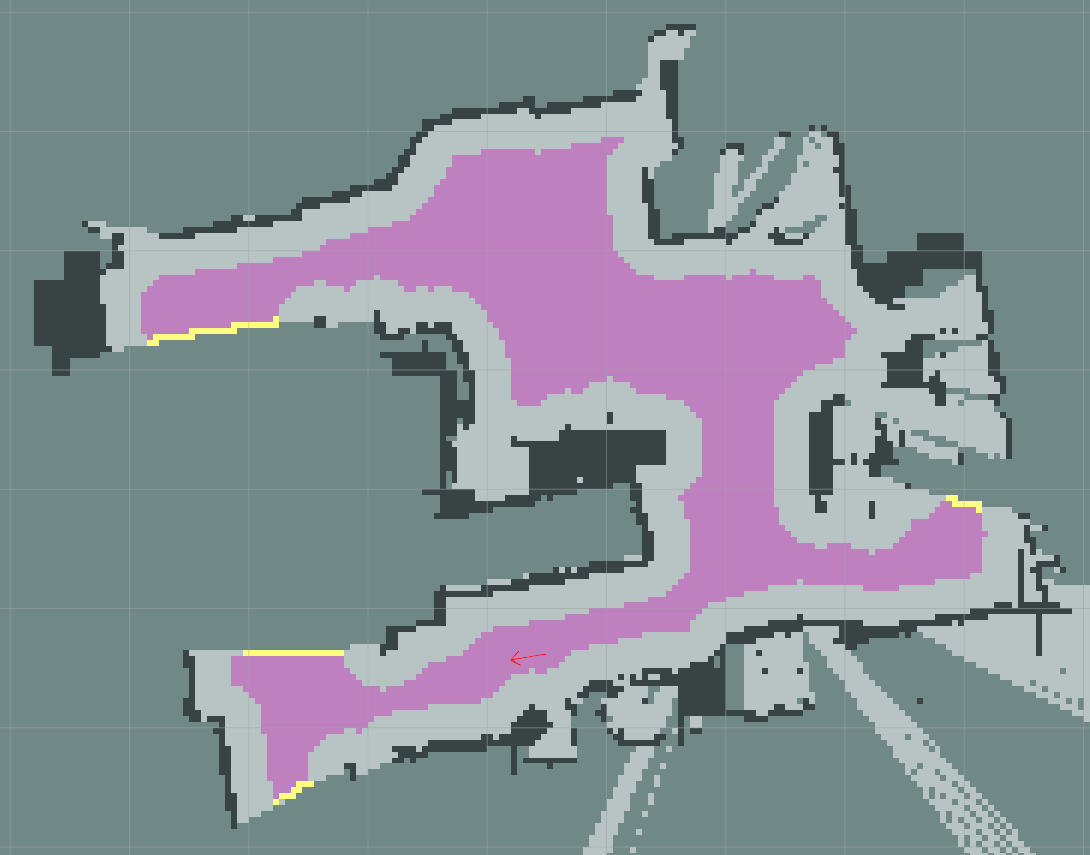
\includegraphics[width=0.9\textwidth]{figures/exploration.png} 
 \caption[Map with accessible cells and frontiers]{A map with accessible cells (purple and yellow cells) and frontiers (yellow cells)}
 \label{fig: exploration}
\end{figure}

Only the current room should be explored. To prevent the robot from driving out of the room during exploration all detected doorways are blocked by virtual obstacles as shown in figure \ref{fig: exploration_door_blocked}. 

If the object detection detects a searched object with a sufficiently high confidence the object is assumed to be found. The estimated location in space is reported and the search is stopped. A decision based on multiple images, like during the search task, is not done during the exploration.

\begin{figure}[h]
 \centering
   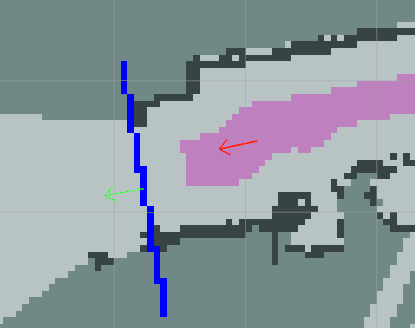
\includegraphics[width=0.7\textwidth]{figures/exploration_door_blocked.png} 
 \caption[Blocked doorway]{Doorway (green arrow) is blocked during exploration}
 \label{fig: exploration_door_blocked}
\end{figure}

\subsection{Search Room Task}

The goal of the search room task is to find an object of the searched type within the current room or to fully search the current room if no searched object is in the room. The low-level planner has to find the best next view pose for the robot to drive to, which minimizes the expected search time, based on the information gathered. It also has to decide if an object was found and if the room was fully searched.

In this work a greedy approach is used to find the best next view pose. The best view pose $\mathbf{p}^*$ is selected by:
\begin{equation}
 \mathbf{p}^*= \argmaxA_{\mathbf{p}} \frac{P(o|\mathbf{p})+B(\mathbf{p})}{T(\mathbf{p}_0,\mathbf{p})}
 \label{search_objective}
\end{equation}

$P(o|\mathbf{p})$ is the probability of finding an object of type $o$ when the robot is at pose $\mathbf{p}$. $B(\mathbf{p})$ is an additional term to promote coverage and is also needed for the termination criteria, as described later. $T(\mathbf{p}_0,\mathbf{p})$ is the time needed to drive from the current pose $\mathbf{p}_0$ to the pose $\mathbf{p}$. $T(\mathbf{p}_0,\mathbf{p})$ is estimated assuming movement on the shortest path between two poses:
\begin{equation}
 T(\mathbf{p}_0,\mathbf{p}) = \frac{|\measuredangle(\mathbf{p}_0,\overrightarrow{\mathbf{p}_0\mathbf{p}})| + |\measuredangle(\overrightarrow{\mathbf{p}_0\mathbf{p}},\mathbf{p})|}{\omega}+\frac{|\overrightarrow{\mathbf{p}_0\mathbf{p}}|}{v}+T_{const}
\end{equation}
$\omega$ and $v$ are the average rotational and translational velocities and $T_{const}$ is a constant time added to account for planning time and other delays.

Estimating the probability $P(o|\mathbf{p})$ is much more difficult. It depends on what is visible when taking an image at pose $\mathbf{p}$, the object probabilities in the visible space and how likely a searched object located in the visible space is detected. Therefore $P(o|\mathbf{p})$ is calculated with:
\begin{equation}
 P(o|\mathbf{p})=\prod_{c \in cells\;in\;room} P(Obj_{c}^{o}|I_{1:t}, \mathbf{x}_{1:t})P(vis_c|\mathbf{p})P(det_c|\mathbf{p})
\end{equation}

Determining visible space is computational expensive and also not really possible in messy environments without a high quality 3D map. Therefore a heuristic is used. This heuristic reduces the problem from 3D to 2D and the limited vertical field of view is ignored. The basic assumption is that an object is visible if viewed from the direction of the nearest accessible location. This is true if objects are side-by-side and not behind each other. The yellow arrows in figure \ref{fig: border_with_dir} show these directions, which are referred to as best directions. The more the direction the cell is viewed from diverges from this best view direction, the less likely the cell is visible. This is modeled with
\begin{equation}
 P(vis_c|\mathbf{p})=\begin{cases}e^{-\frac{\measuredangle(\mathbf{p},\overrightarrow{\mathbf{p}c})^2}{2*\sigma_{view}^2}} & if\;in\;field\;of\;view \\ 0 & else \end{cases}
\end{equation}

\begin{figure}[h]
 \centering
   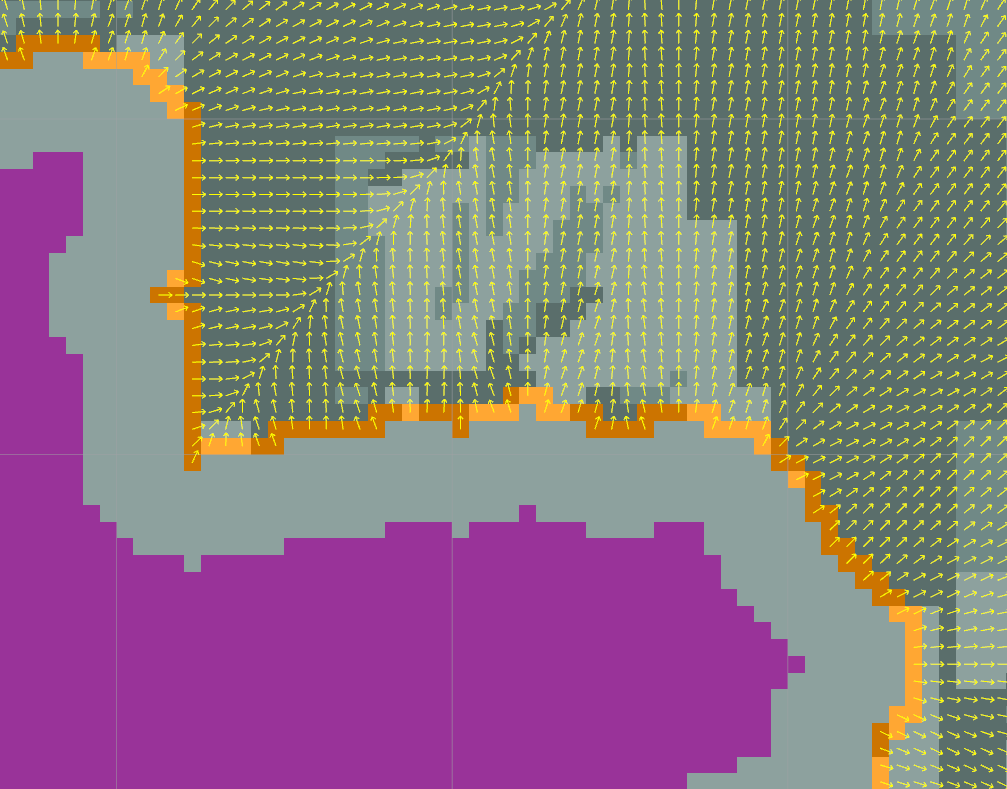
\includegraphics[width=0.7\textwidth]{figures/border_with_dir.png} 
 \caption[Best directions to view cell]{Best view directions (yellow arrows), accessible area (purple), border of free space (orange) and 2D grid map in background} 
 \label{fig: border_with_dir}
\end{figure}

This model of visibility is very pessimistic as many objects are also visible from other view angles. To reduce the number of unnecessary views cells seen more often than a threshold value are assumed to be sufficiently viewed and ignored in later probability calculations. 

The used estimate of the probability of detecting the object depending on its location relative to the robot is shown in figure \ref{fig: detection_kernel}. Near cells are weighted higher as small objects are difficult to detect from far away. Large objects on the other hand occupy multiple cells and therefore view poses covering the whole object are implicitly preferred. At the edge of the field of view successful object detections are less likely, which is also taken into account.

\begin{figure}[h]
 \centering
   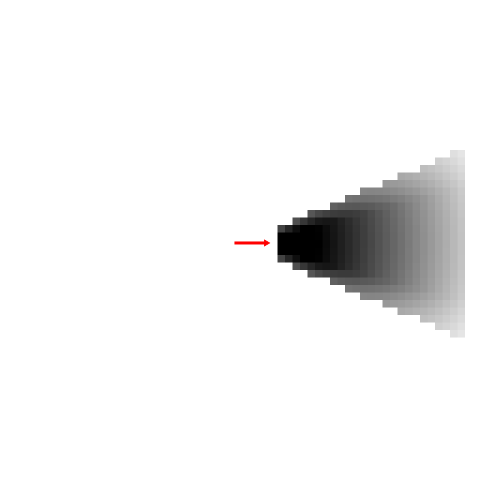
\includegraphics[width=0.4\textwidth,trim= 230 130 0 130,clip]{figures/detected_kernel.png} 
 \caption[Detection probabilities in field of view]{Probabilities for detecting the object depending on the location relative to the robot (red arrow); the probability of cells is 1 for black cells and 0 for white cells} 
 \label{fig: detection_kernel}
\end{figure}

To find the best next view pose sample poses are generated at regular x and y distances with multiple different orientations. A sample pose is valid if it is at an accessible location and was not visited before. From the valid sample poses the best is chosen based on equation \ref{search_objective}.

The check if an object was found is done in two different ways. On the one hand an object is said to be found if a sufficiently confident detection was made by the object detection CNN. In this case the location is estimated based on the position in the image and the depth values of the detection. This location is the result of the search and the search is stopped. On the other hand the probability of an object being in a grid cell is also estimated like in section \ref{sec:Object Mapping}. Here the performance is not as much a concern. This is the case as only one object type is of interest and the localization is assumed to be accurate after exploration, so the creation of the probability map has not to be done for multiple particles. Therefore more detection samples can be used leading to more reliable results. If the probability of a searched object being in a cell is higher than a threshold, the object is assumed to be found and the respective cell is the result of the search task.

In case no object can be found the planner needs to decide if the room was fully searched. It is impossible for the system to decide which cells in a room can possibly be seen, at least based on the generated 3D map. Therefore another heuristic is used to define a termination criteria. Above the assumption was made that a cell is seen from the nearest accessible cell. In reverse this means the room is fully searched if the robot has looked outward at every accessible cell. To achieve this a set of cells enclosing the accessible area is created and the direction from the nearest accessible cell to this border is calculated for every cell in this set. This is shown in figure \ref{fig: border_all} 
\begin{figure}[h]
 \centering
   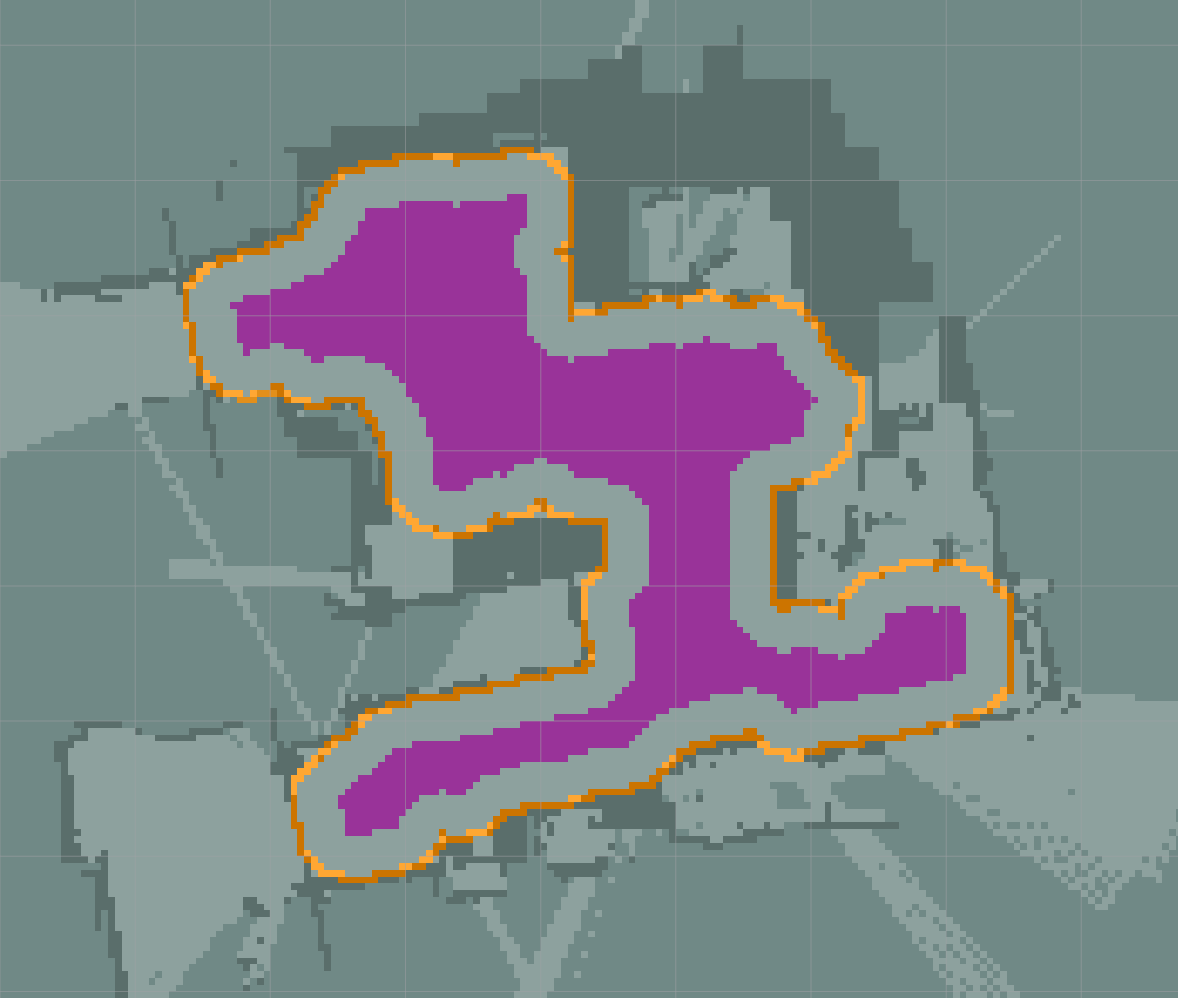
\includegraphics[width=0.9\textwidth]{figures/border_all.png} 
 \caption[Direction of search border]{Best view directions (yellow arrows), accessible area (purple), border of free space (orange) and 2D grid map in background}
 \label{fig: border_all}
\end{figure}
In addition every cell in the set gets a counter. When the object detection is run on an image all cells of the border in the field of view of the camera with an orientation similar to the direction the image is taken are increased by one. This is illustrated in figure \ref{fig: border_view}.
\begin{figure}[h]
 \centering
   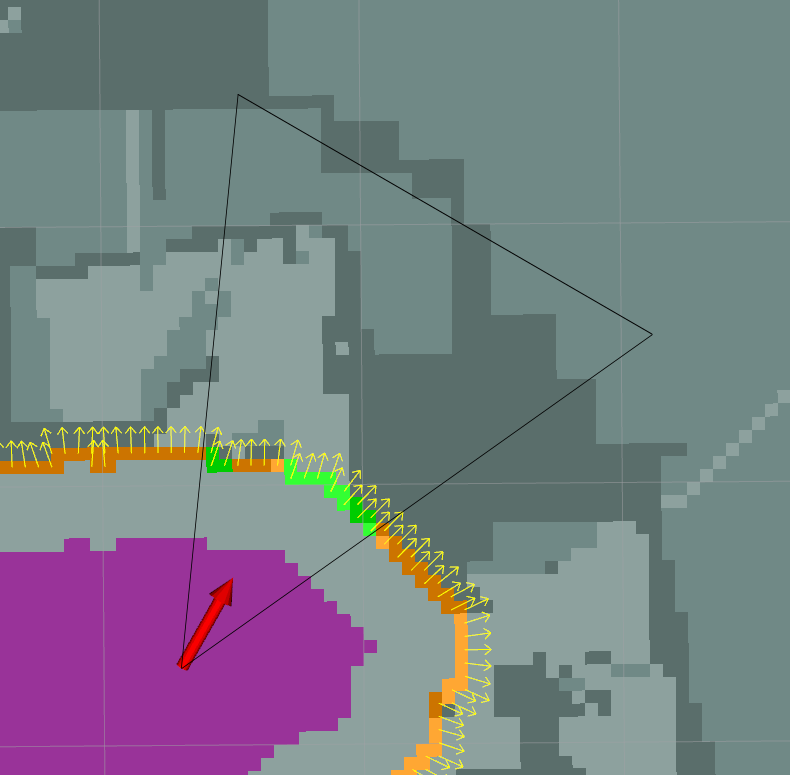
\includegraphics[width=0.7\textwidth]{figures/border_view.png} 
 \caption[Search border update]{Update of border cell counter: Only cells within the field of view (black triangle) and having a similar orientation as the camera (red arrow) are updated (green cells); other cells on the border are not updated (orange cells)}
 \label{fig: border_view}
\end{figure} 
Based on this the term $B(\mathbf{p})$ is calculated with:
\begin{equation}
 B(\mathbf{p})=\begin{cases} V_B|\mathbf{C_{B_{interest}}}| & if\;|\mathbf{C_{B_{interest}}}| > 0 \\ -\infty & else \end{cases}
\end{equation}
$\mathbf{|C_{B_{interest}}}|$ is the number of border cells, whose counter would be increased in a view from pose $\mathbf{p}$ and is lower than a threshold parameter. $V_B$ is a parameter weighting coverage versus finding probability. Ultimately the termination criteria is defined with $P(o|\mathbf{p}^*) \leq 0 \wedge B(\mathbf{p}^*) \leq 0$.  

